In the following sequence diagrams, we are going to explain and represent the interactions that happen between the main components of CLup. This is still a high-level description of the actual interactions that will be developed. Thus function names, results, errors, and other details will be modified or added during the development process. 

\begin{figure}[H]
    \centering
    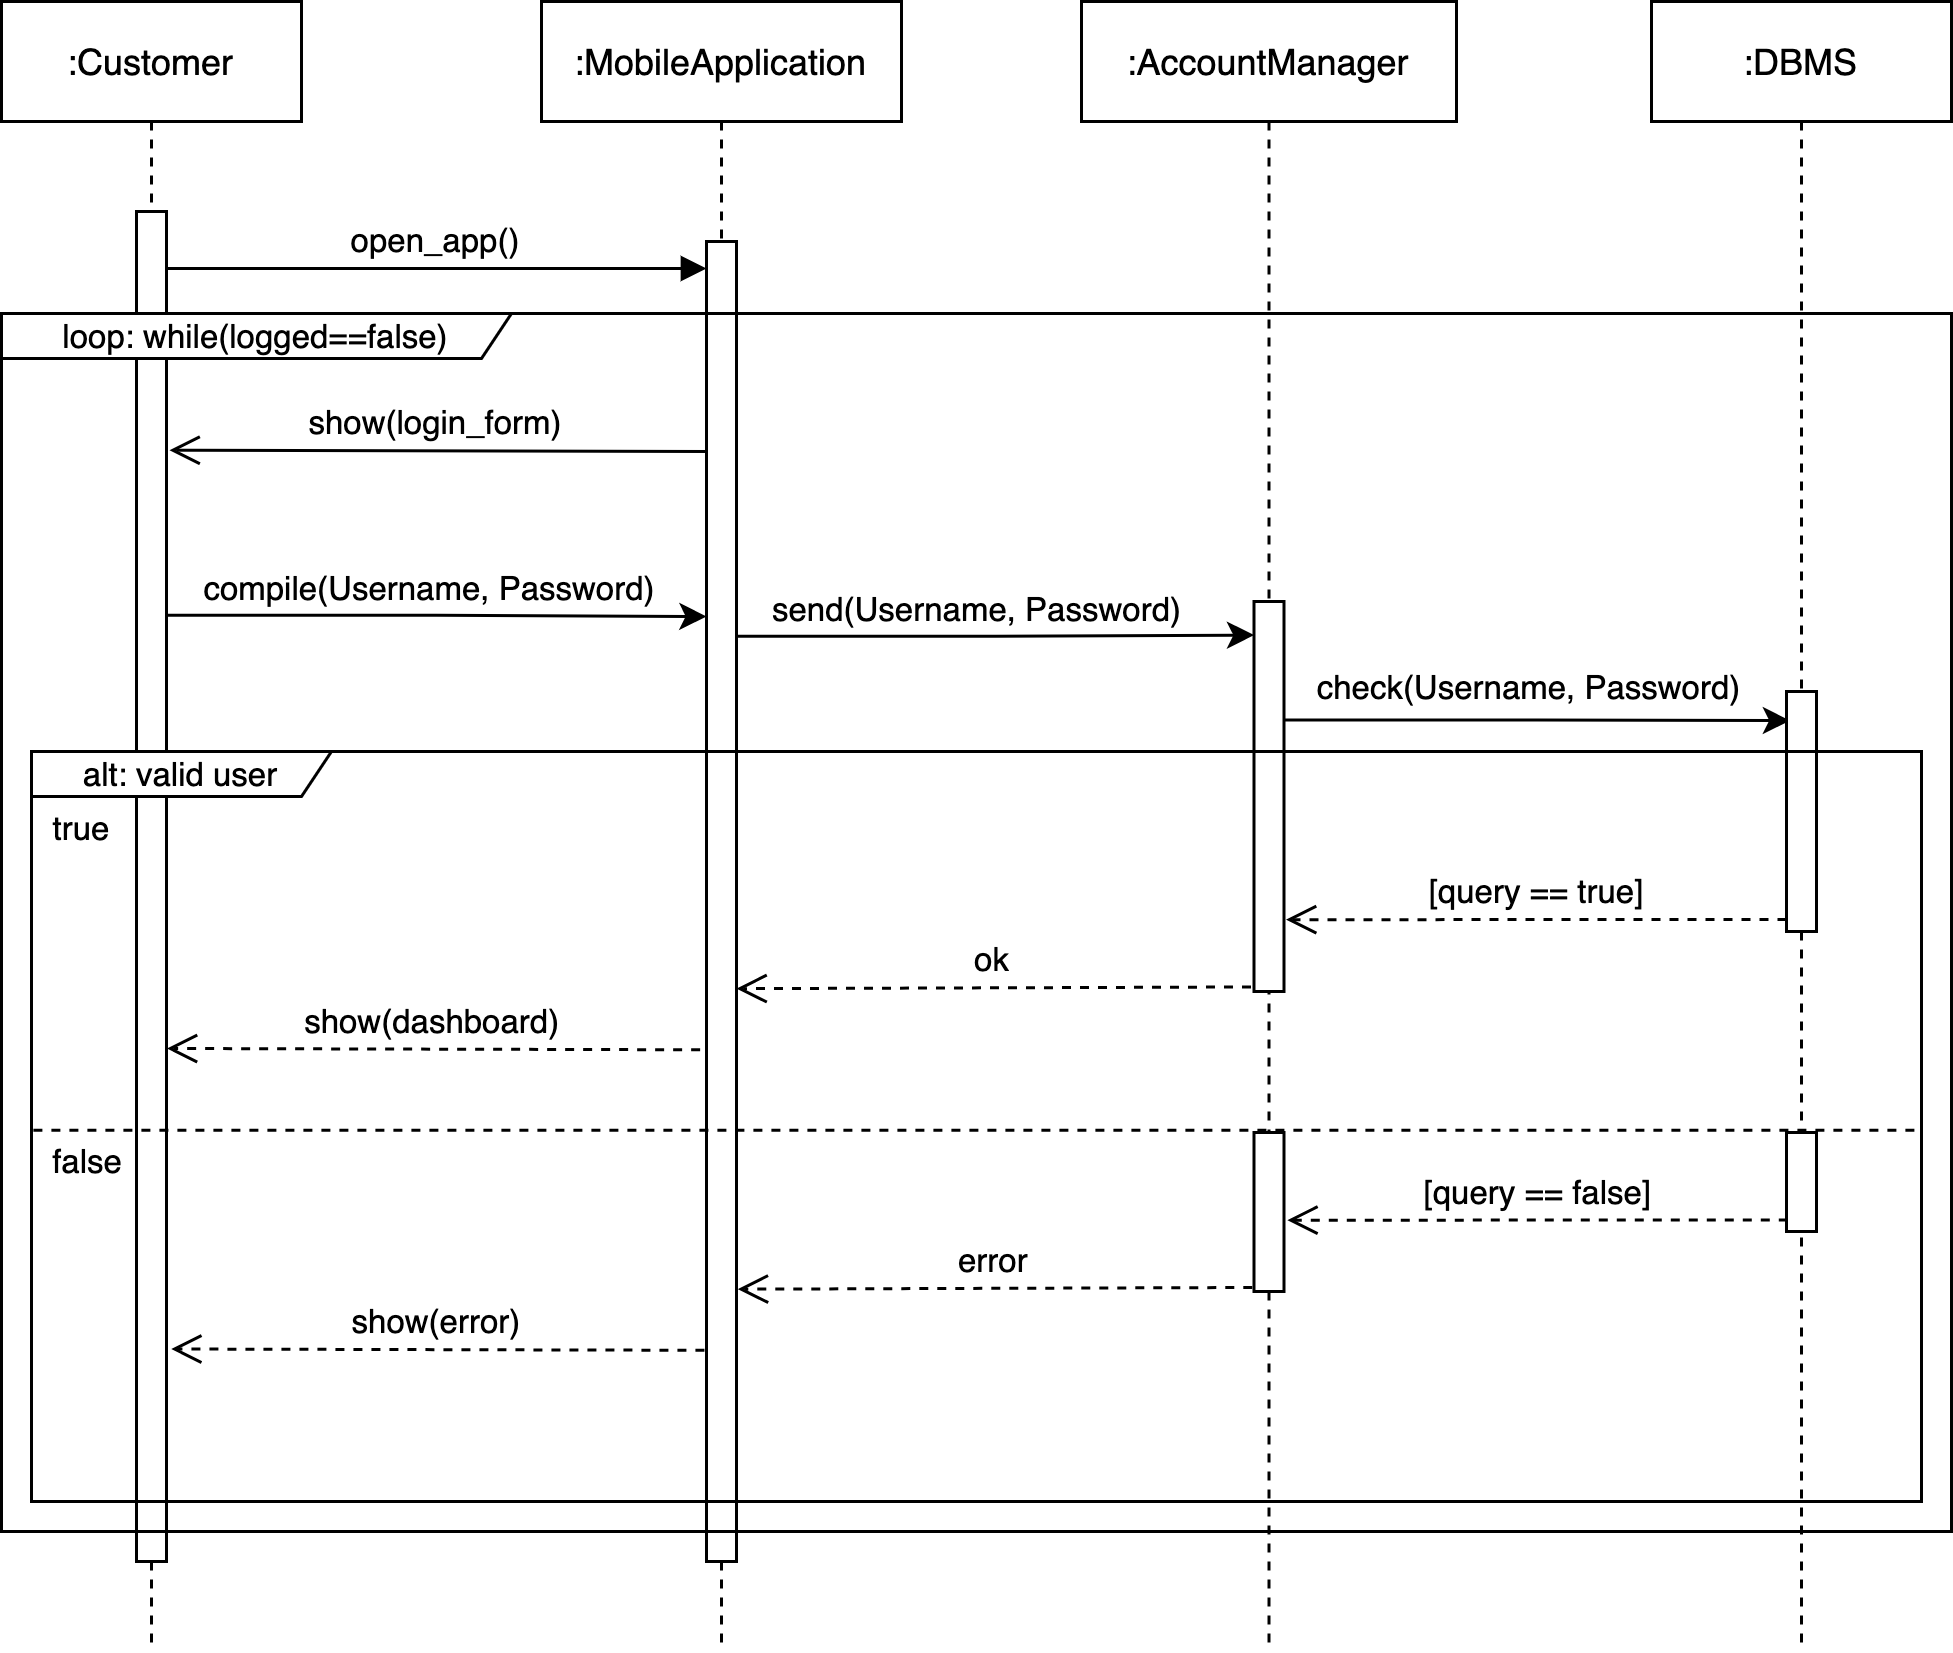
\includegraphics[width=16cm]{runtime_view-Login.png}
    \caption{Customer Login}
\end{figure}

\begin{figure}[H]
    \centering
    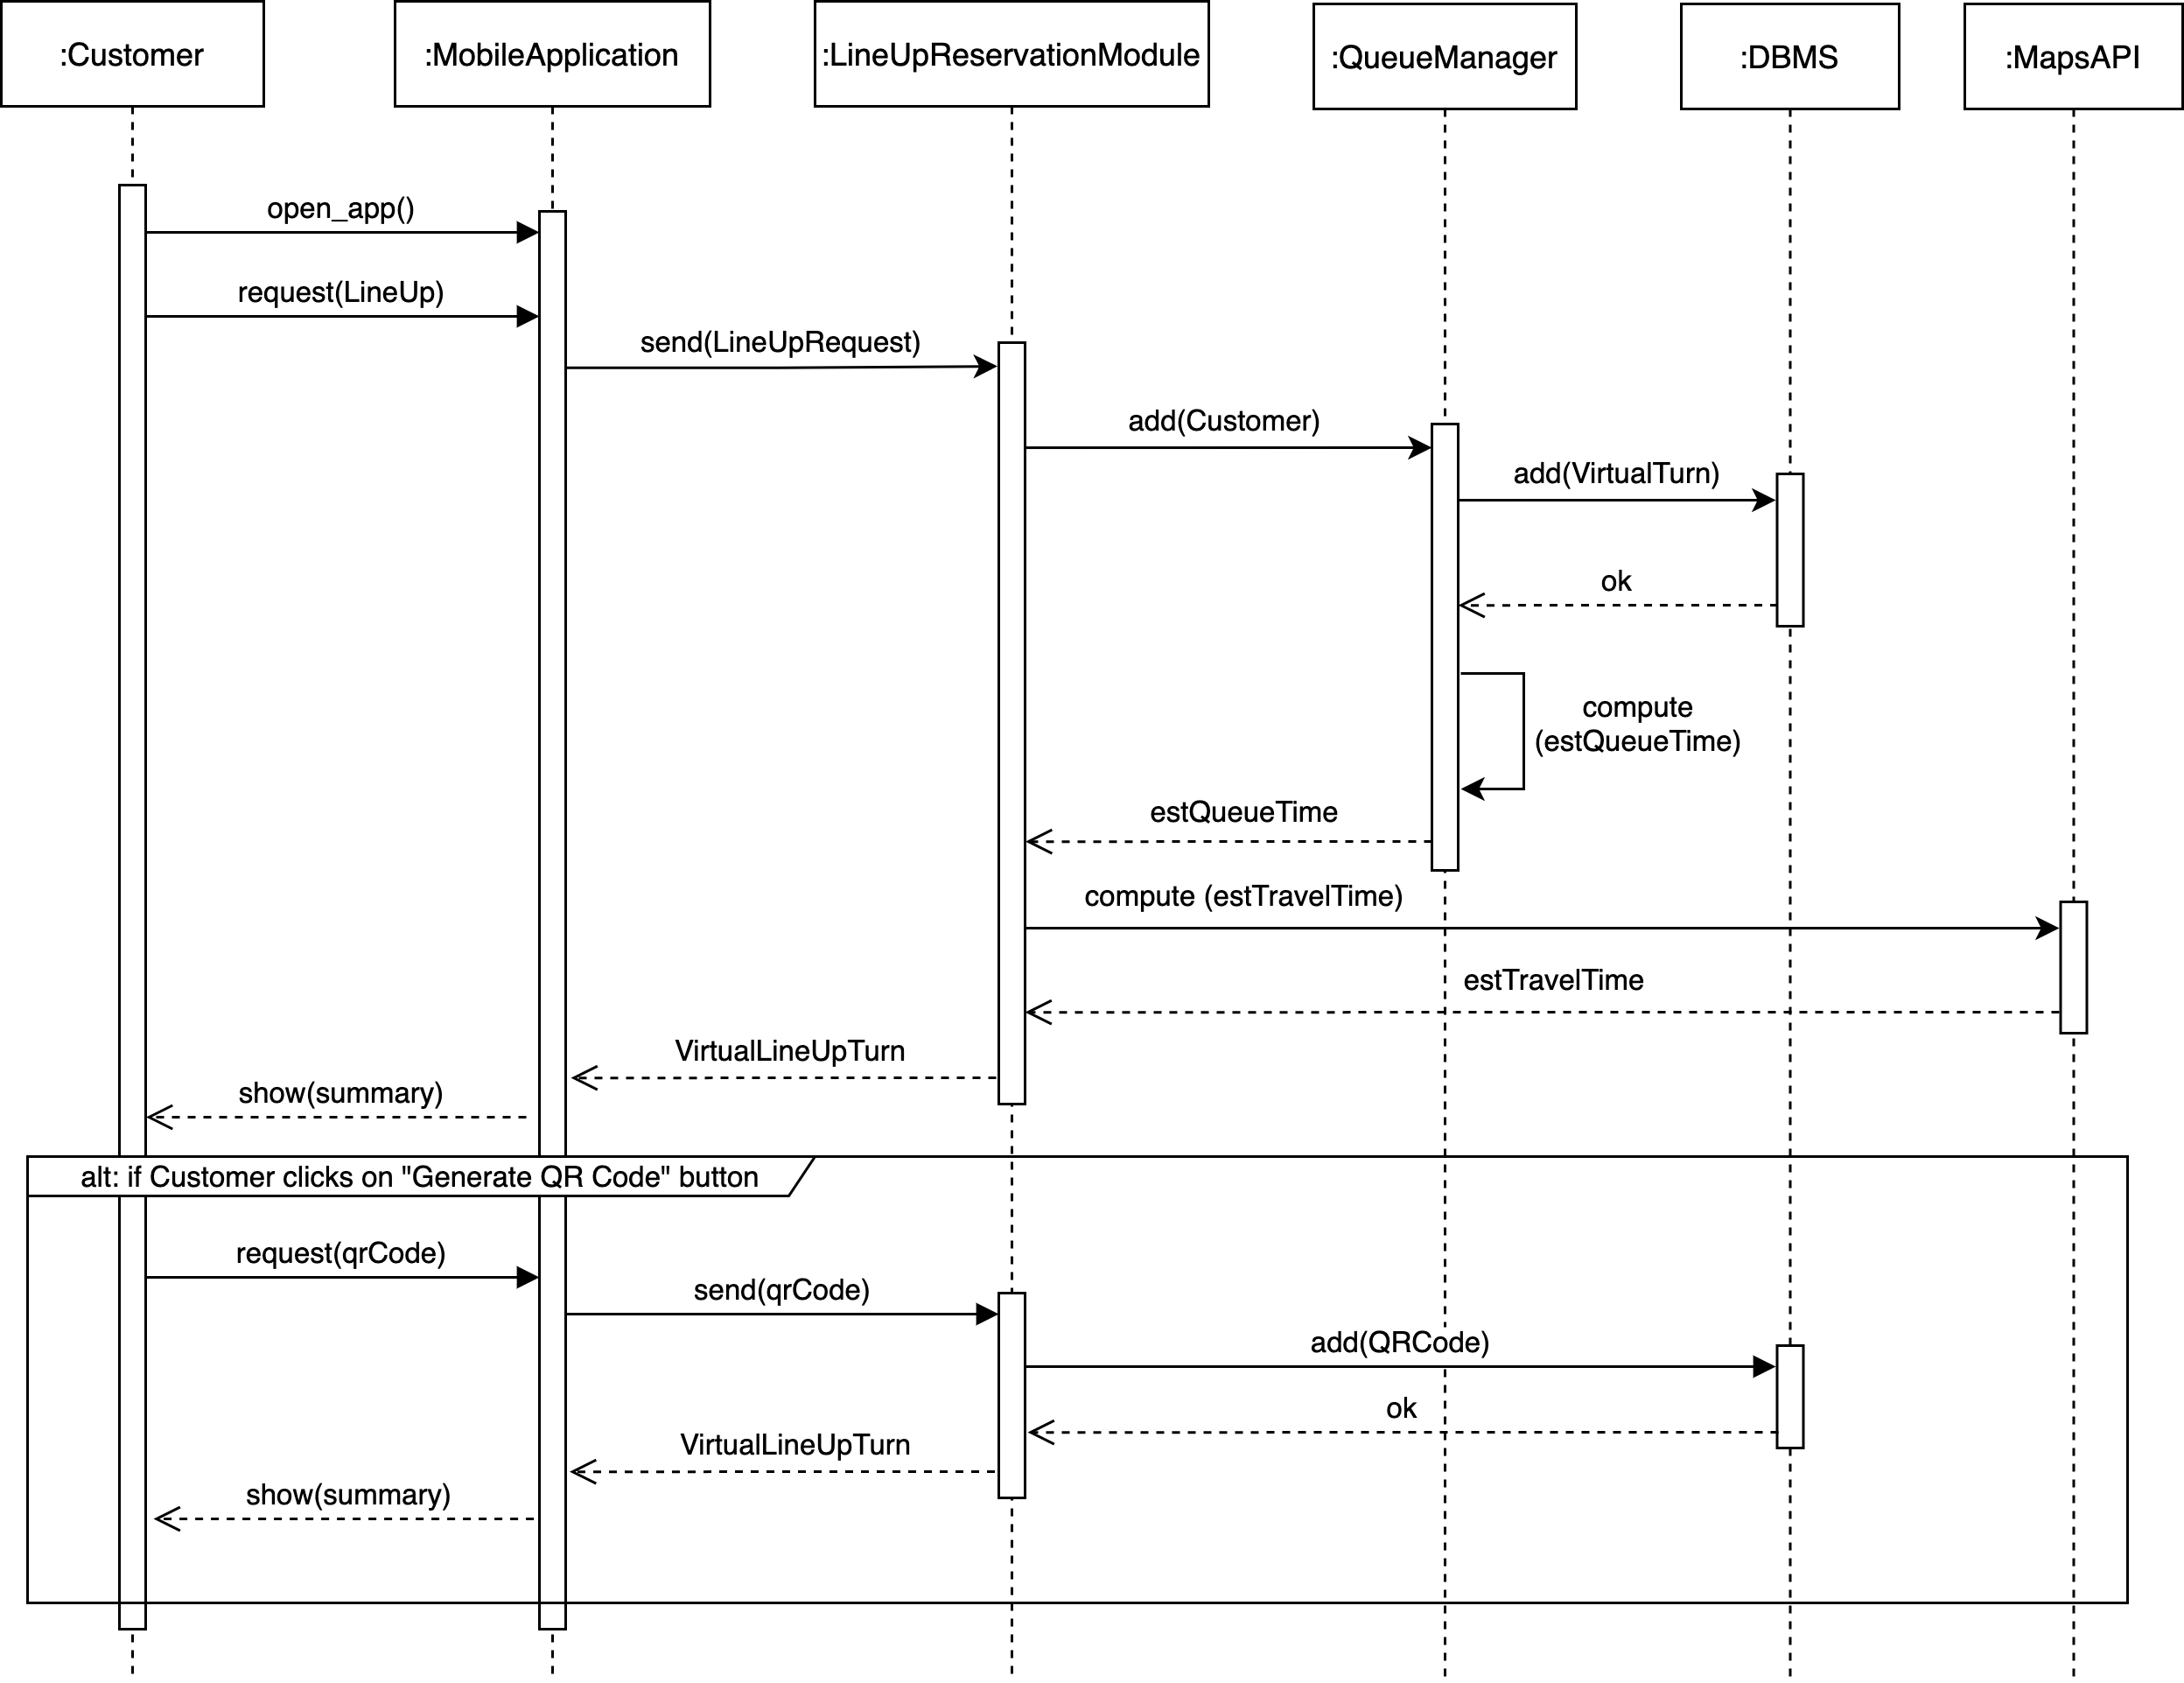
\includegraphics[width=16cm]{runtime_view-LineUpApp.png}
    \caption{Lineup via application}
\end{figure}

\begin{figure}[H]
    \centering
    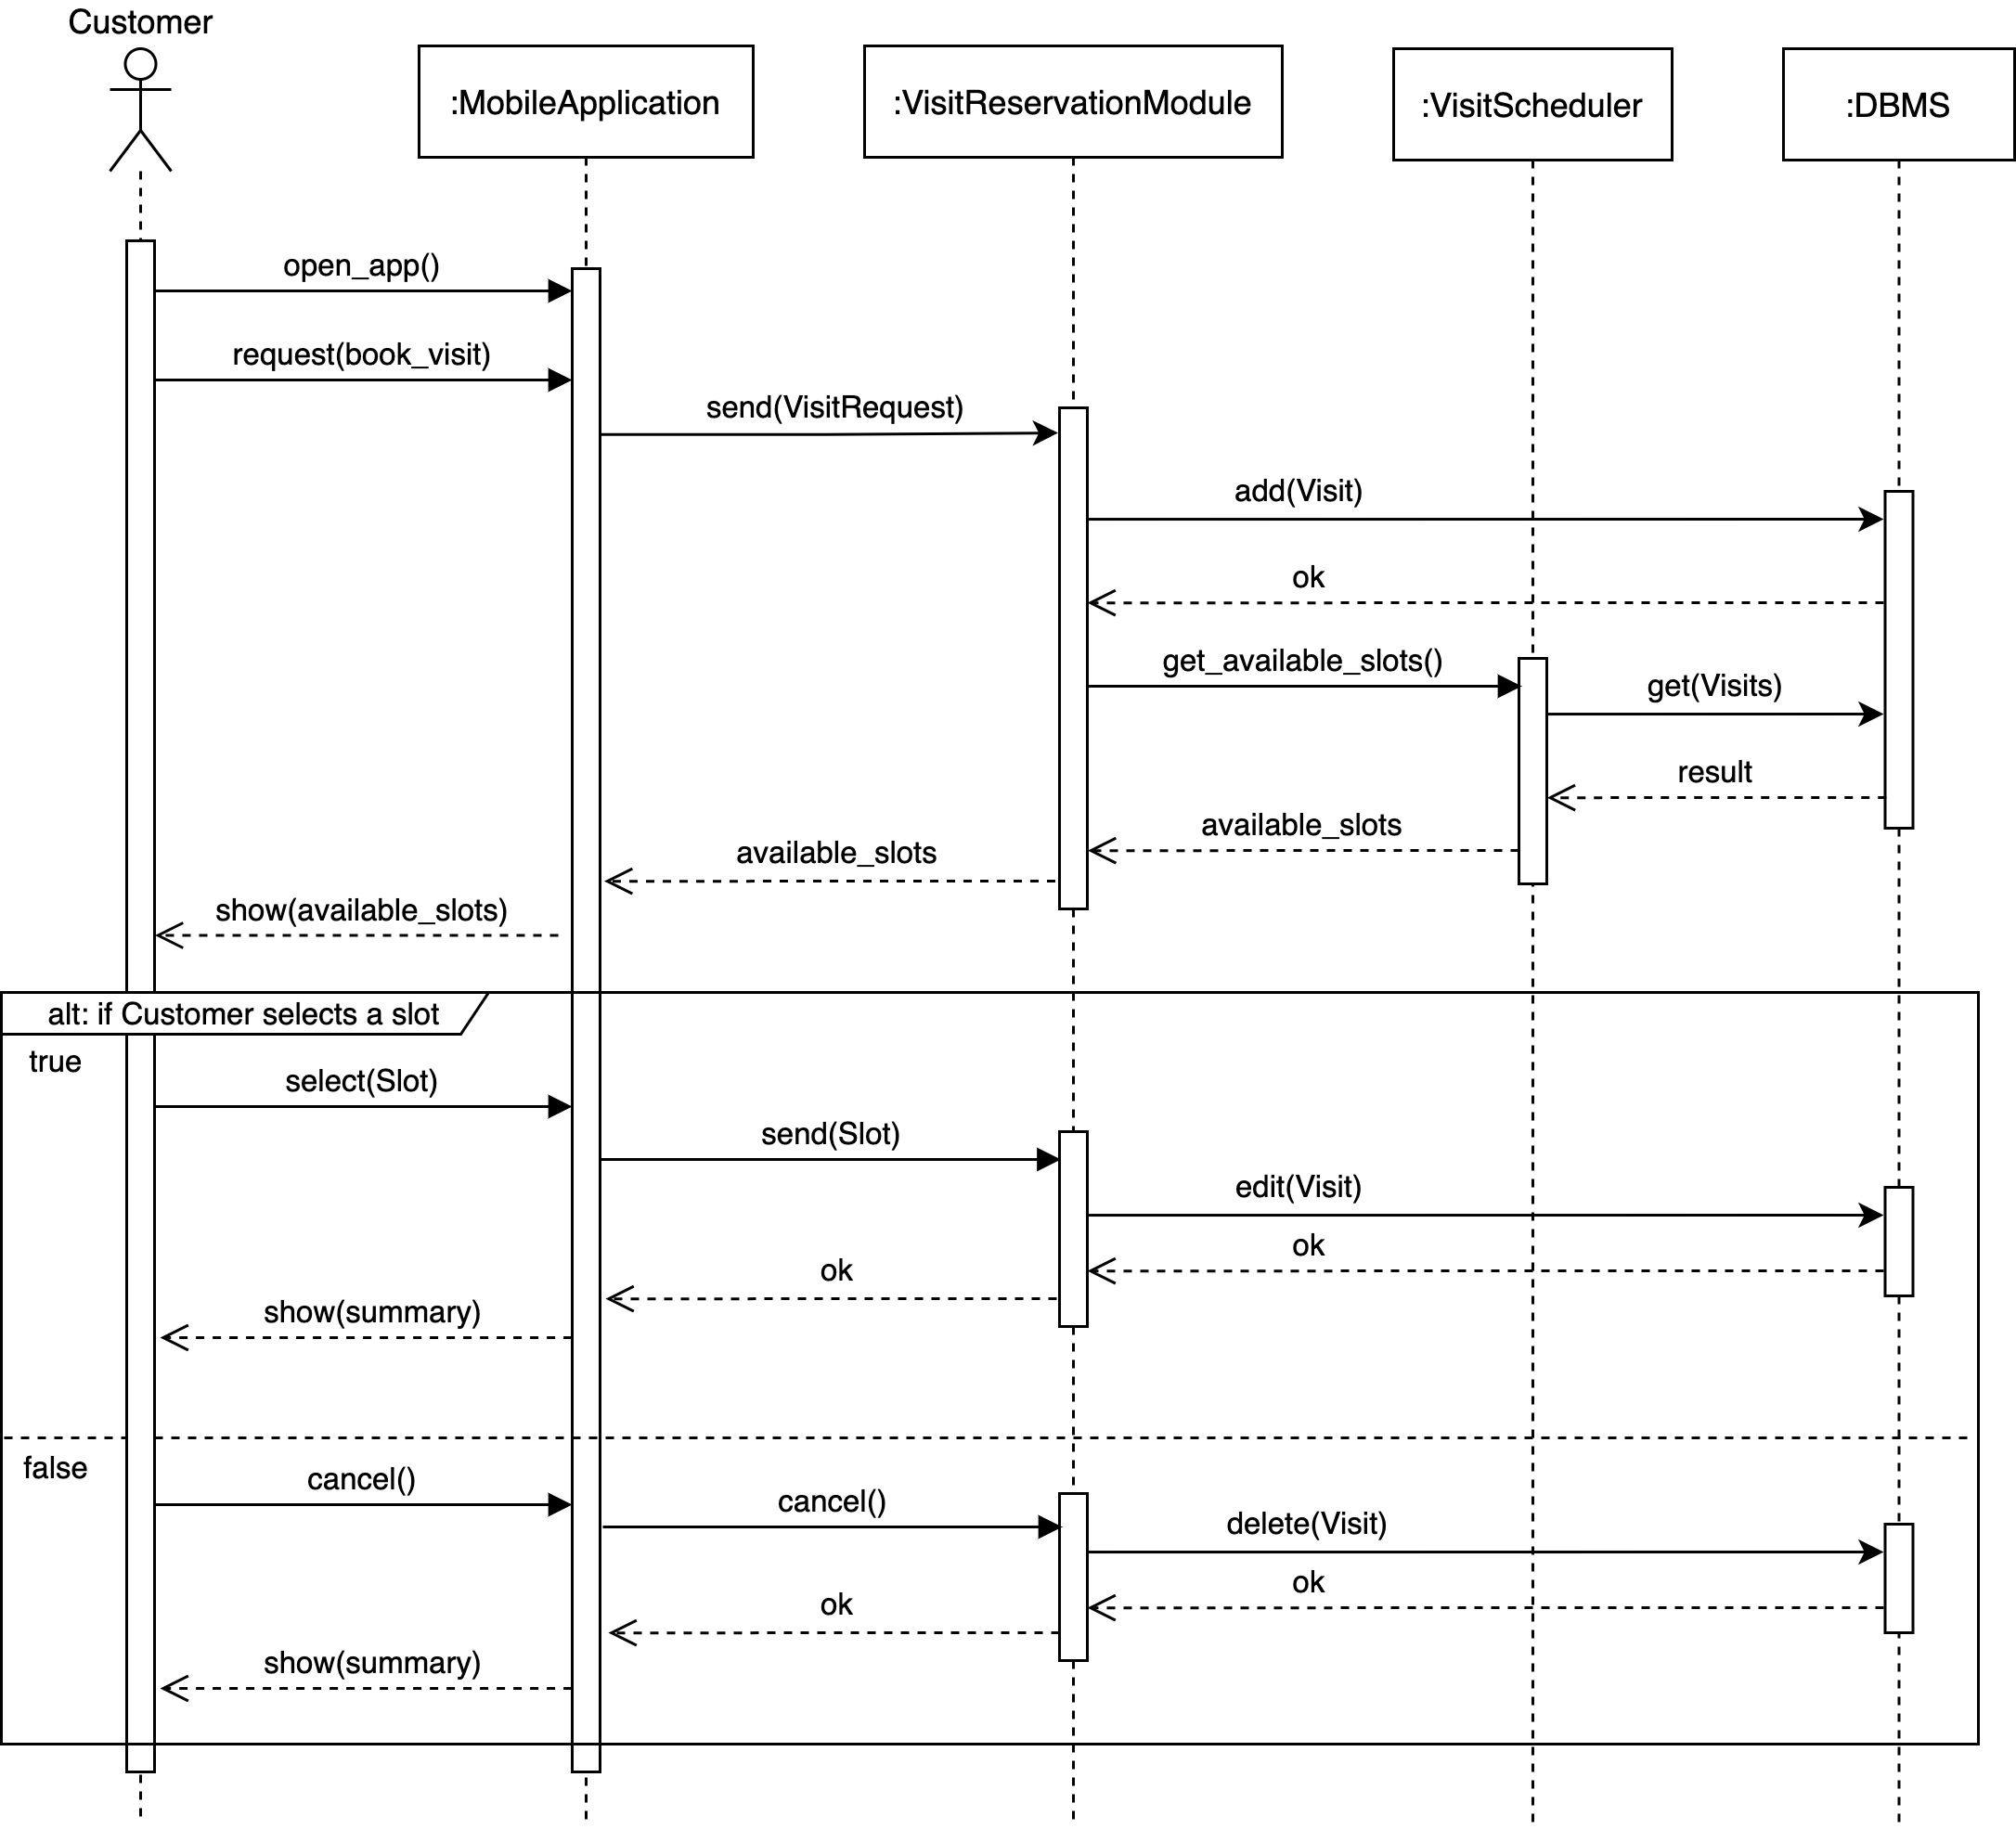
\includegraphics[width=16cm]{runtime_view-BookVisit.png}
    \caption{Book a visit}
\end{figure}

\begin{figure}[H]
    \centering
    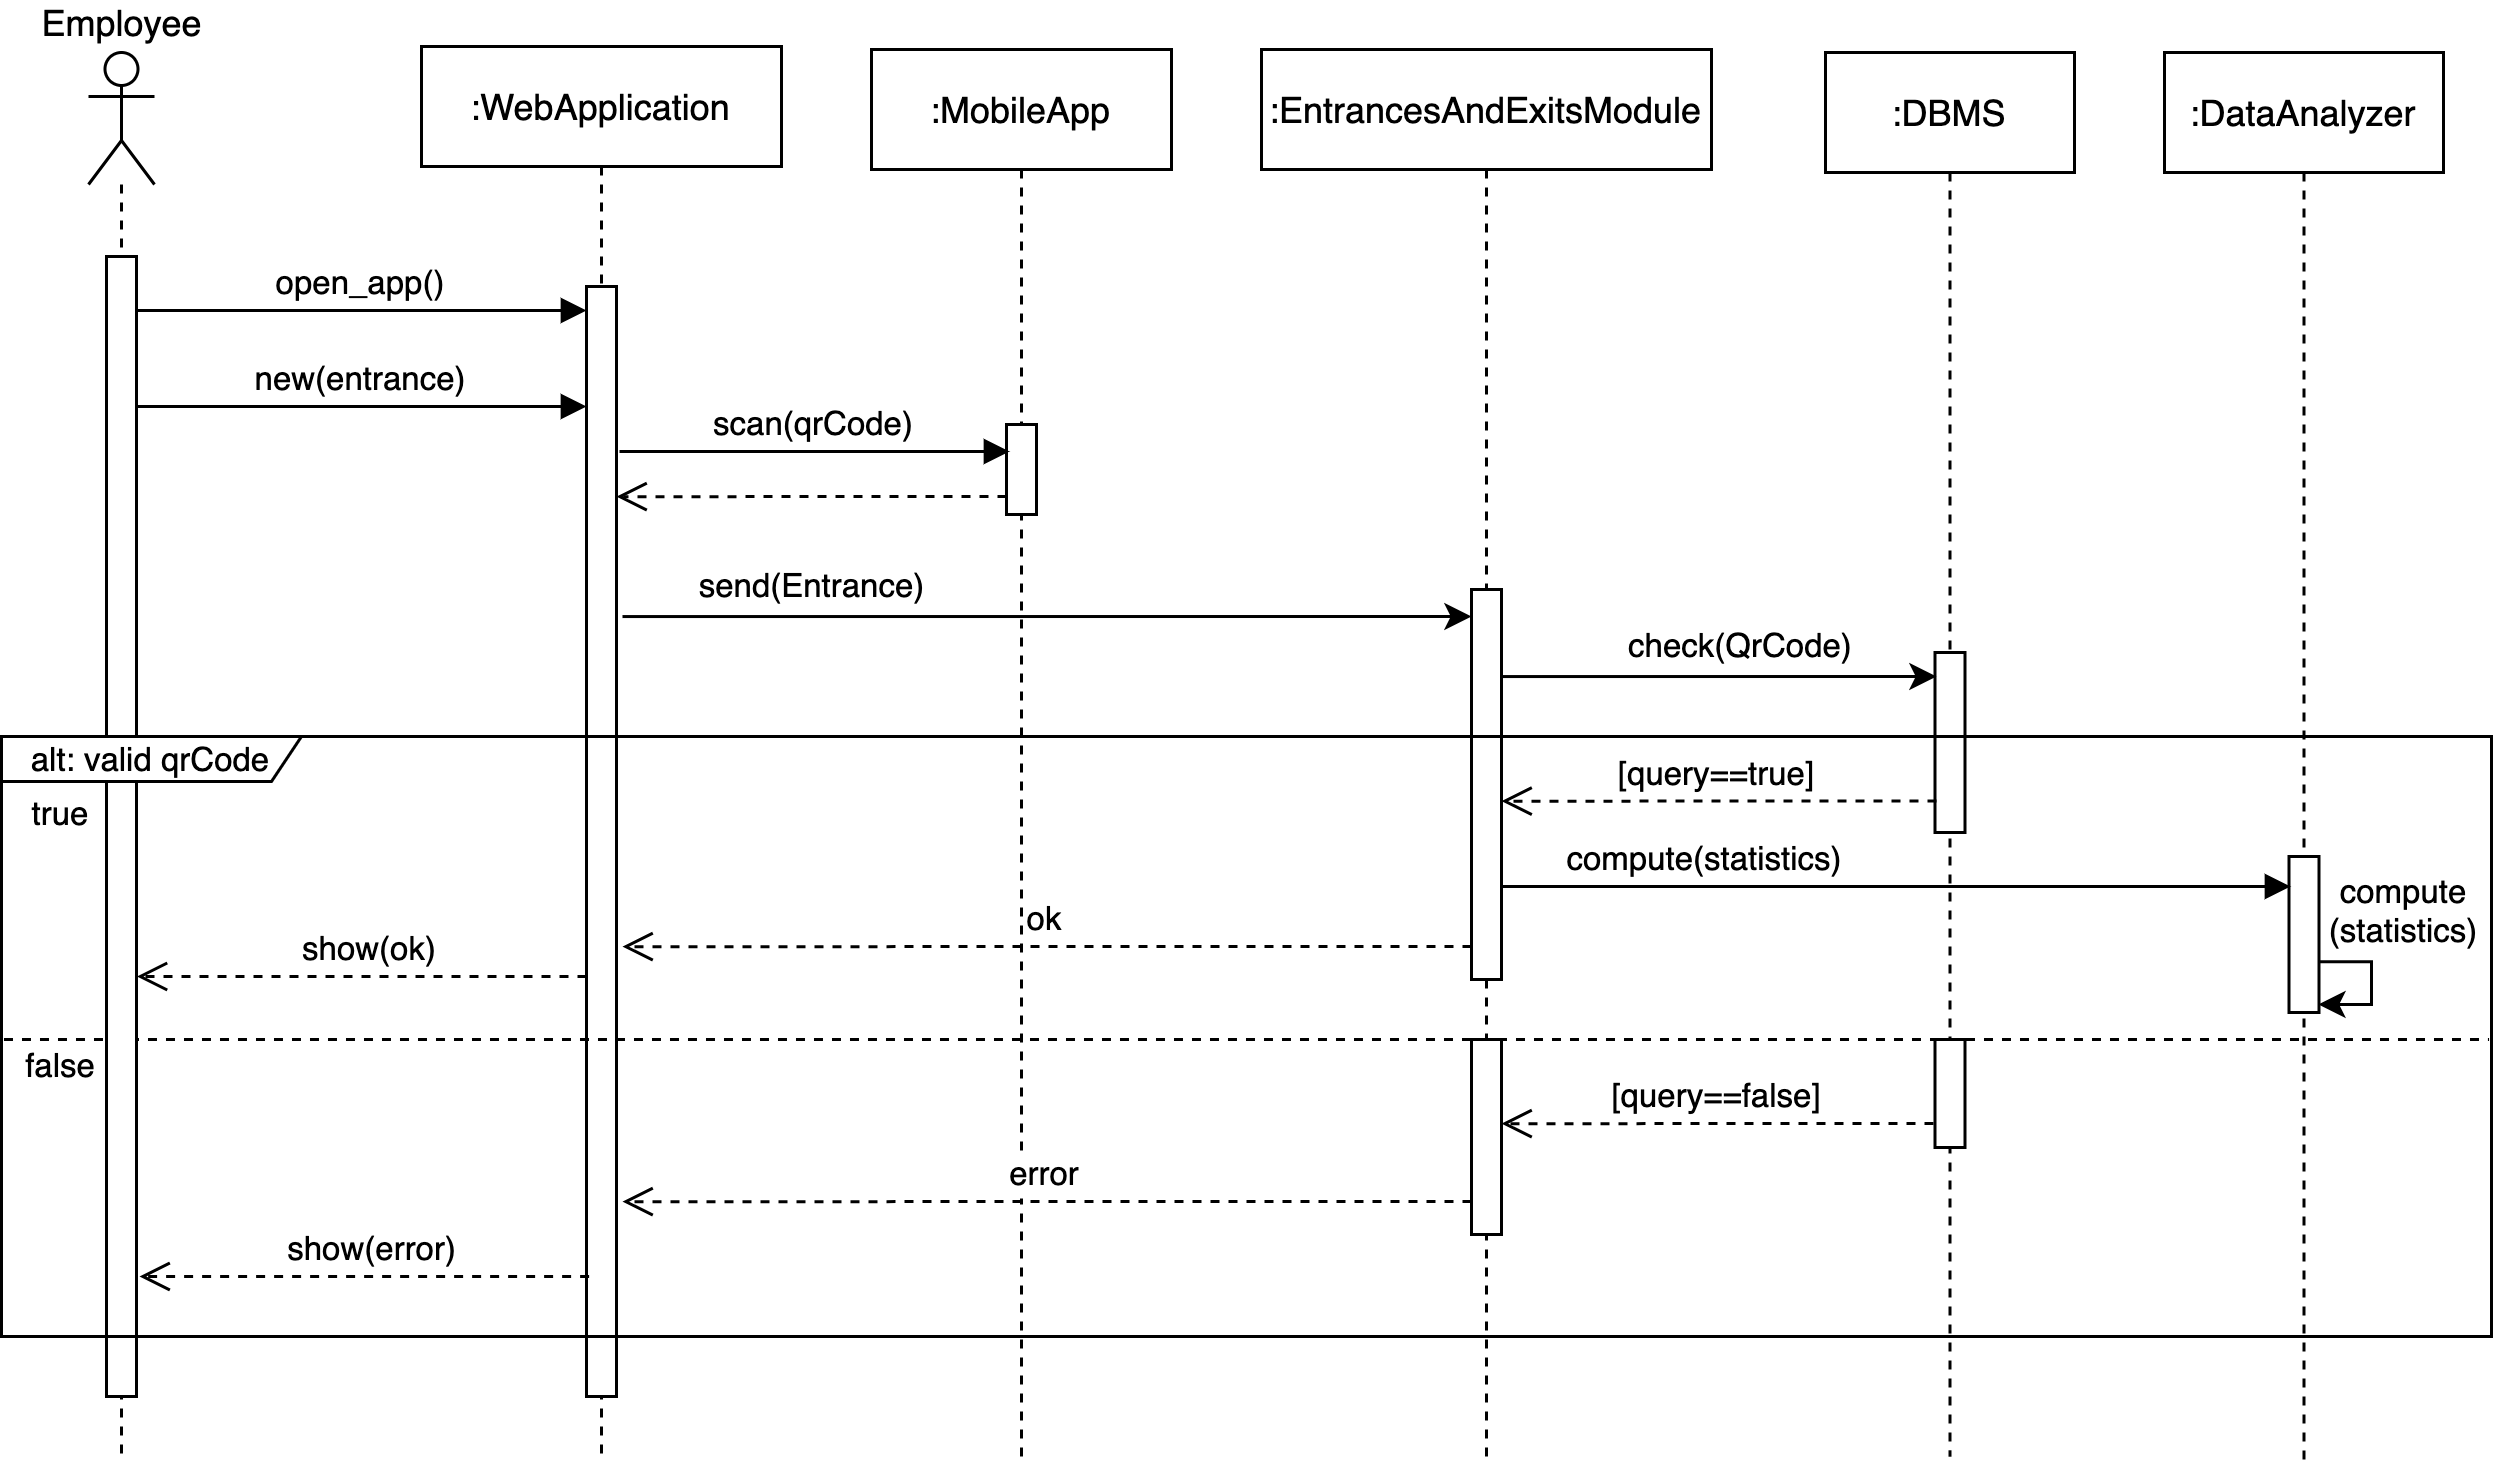
\includegraphics[width=16cm]{runtime_view-qrCodeEntrance.png}
    \caption{Entrance with a QR Code}
\end{figure}

\begin{figure}[H]
    \centering
    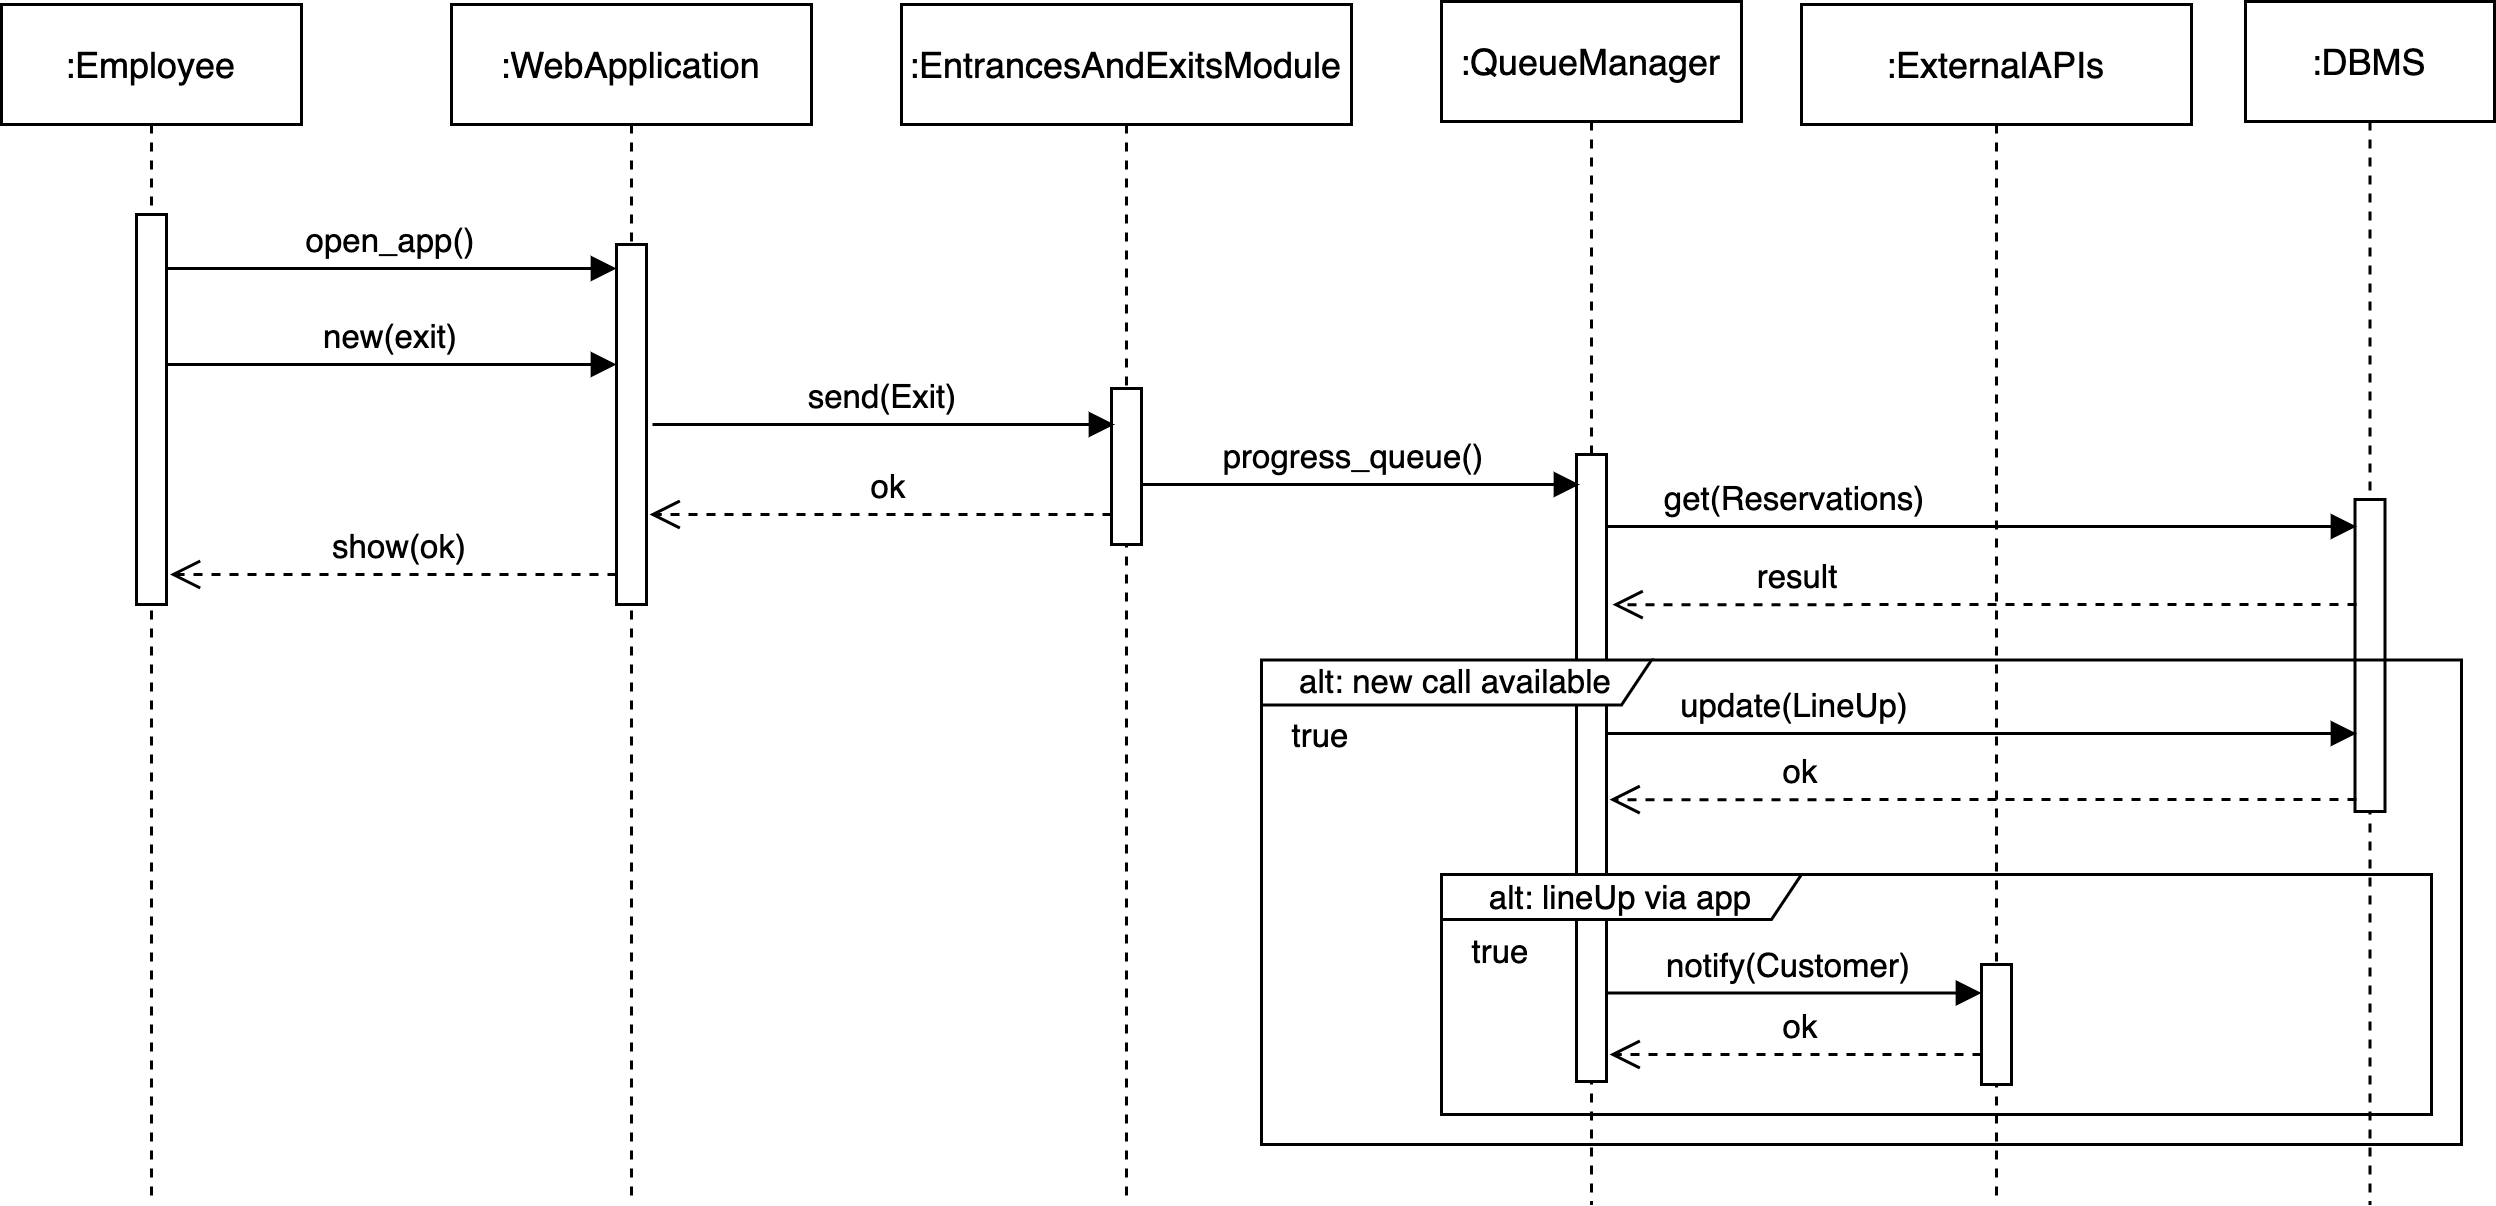
\includegraphics[width=16cm]{runtime_view-ReportExit.png}
    \caption{Exit report}
\end{figure}

\begin{figure}[H]
    \centering
    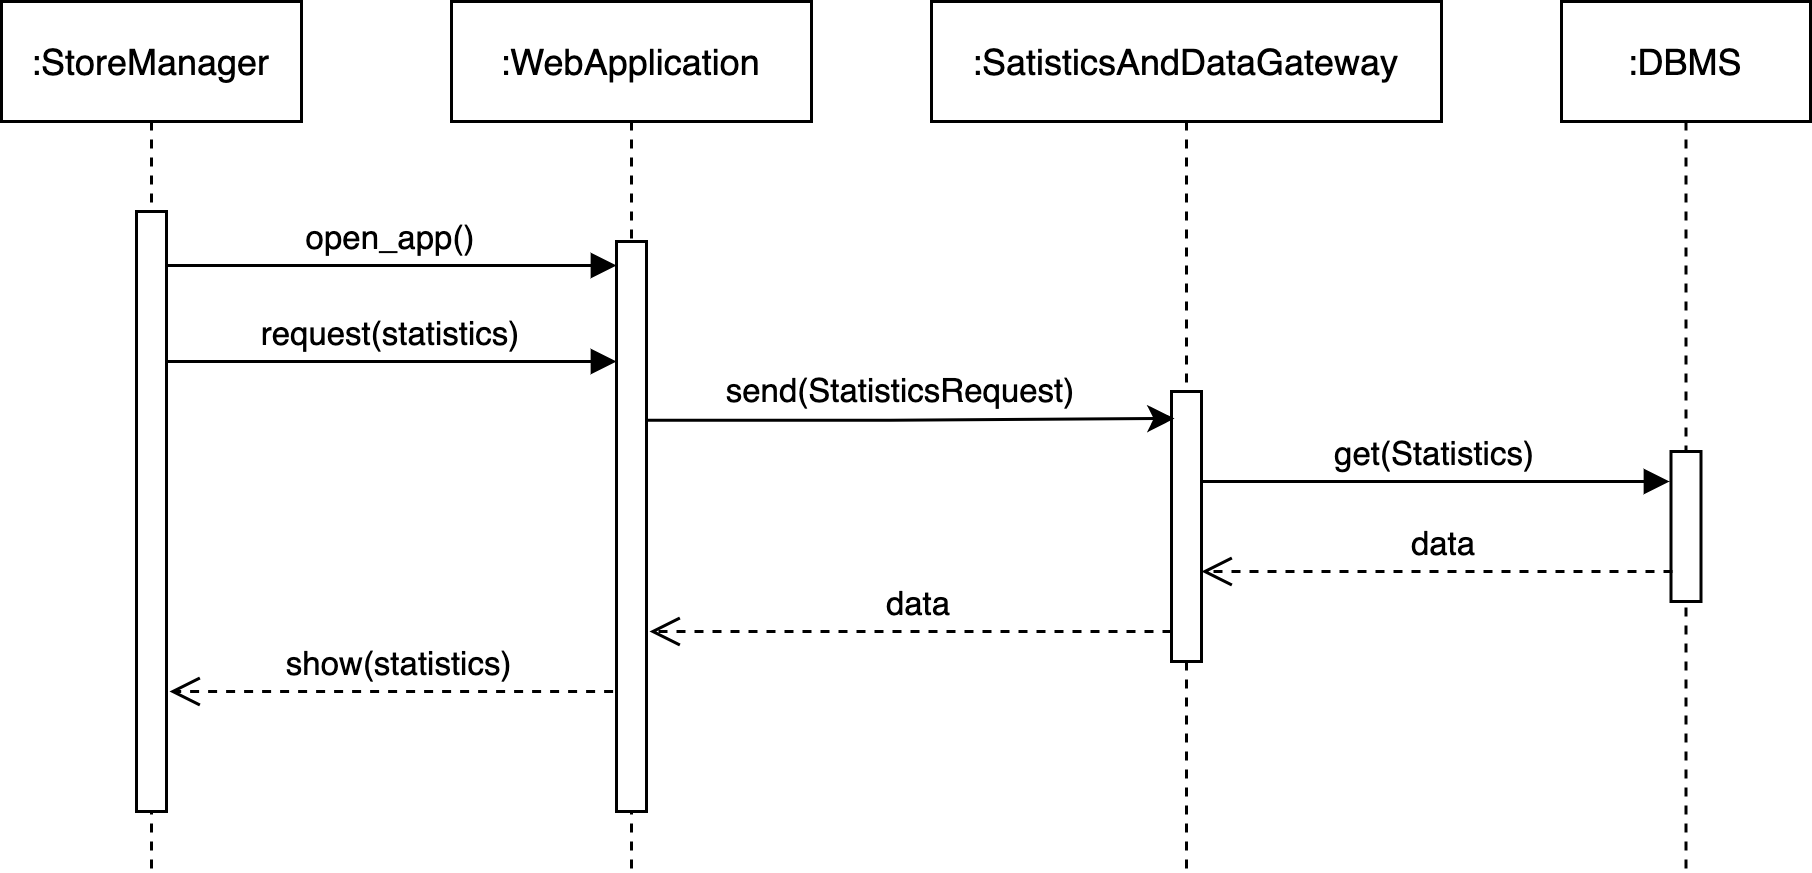
\includegraphics[width=16cm]{runtime_view-Statistics.png}
    \caption{Statistics and charts visualization}
\end{figure}